\documentclass[12pt]{scrartcl}

\usepackage[utf8]{inputenc}
\usepackage[letterpaper]{geometry}
\usepackage{fancyhdr}
\usepackage{csquotes}
\usepackage[french]{babel}
\usepackage{graphicx}
\graphicspath{ {./images_rapport/} }

\pagestyle{fancy}
% \fancyhead[R]{} - Active if we don't want the base fancy header
\fancyfoot[L]{INF1900}
\fancyfoot[R]{Librairies et débogage}

\author{Laurent Bourgon \\Mehdi Benouhoud \\Ihsane Majdoubi \\Catalina Andrea Araya Figueroa}
\subtitle{Travaux pratiques 7 et 8}
\title{Production de librairie statique et stratégie de débogage}

\date{Lundi 13 mars 2023}


\begin{document}
\maketitle



\newpage

\section{Description de la librairie}

\subsection{Classes}
\subsubsection{Led}
Depuis le début du cours, nous utilisons un diode électro-luminescente située
sur le circuit imprimé du robot. Cette diode est dite  \textquote{bi-colore}, c'est-à-dire
qu'elle peut s'allumer en rouge ou en vert, dépendament du sens du courant qu'on
lui transmets. En faisant clignoter rapidement la diode en alternant la couleur,
on obtient une troisième couleur: ambrée.

\begin{figure}[h]
    \centering
    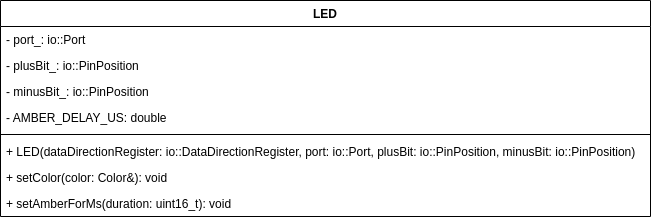
\includegraphics[scale=0.75]{LED_diagramme_classe}
    \caption{Diagramme de classe UML de \textbf{Led}}
\end{figure}

La classe est doté d'un constructeur, nous permettant d'indiquer où est branchée
la diode.
\begin{verbatim}
    Led(io::DataDirectionRegister dataDirectionRegister, io::Port port,
        const io::PinPosition plus, const io::PinPosition minus)
\end{verbatim}

\verb|dataDirectionRegister| indique le registre de direction des données où la
diode est branchée, \verb|port| indique son port et finalement
\verb|plus| et \verb|minus| indique les broches sur lesquelles sont branchés la
respectivement cathode et l'anode de la diode. Il est important de respecter ce
sens afin de permettre à la méthode \verb|setColor(const Color &color)| de
fonctionner adéquatement.
\\ \\
La méthode \verb|setColor(const Color &color)| permet d'allumer la diode en rouge
ou en vert, en passant en paramètre \verb|Color::RED| ou \verb|Color::GREEN|.
\\ \\
La méthode \verb|setAmberForMs(const uint16_t durationMs)| permets d'allumer la
diode en ambrée. Nous devont passer une durée (en milisecondes) en paramètre. En
effet, puisque la diode doit alterner rapidement entre le rouge et le vert, il
est impossible d'effectuer cette opération indéfiniement.
% TODO Peut-être mieux expliquer pourquoi on peut pas faire ça?
\newpage
\section{Modifications apportées au \textit{Makefile} de départ}

\end{document}